\documentclass[helvetica]{seminar} 
\input{xy}
\xyoption{all}
\usepackage{graphicx} 
\usepackage{slidesec} 
\usepackage{url}
\usepackage[normalem]{ulem}
\usepackage[usenames]{color}

\long\def\symbolfootnote[#1]#2{\begingroup%
\def\thefootnote{\fnsymbol{footnote}}\footnote[#1]{#2}\endgroup}

% to fix problems making landscape seminar pdfs
% Letter...
\pdfpagewidth=11truein
\pdfpageheight=8.5truein
\pdfhorigin=1truein     % default value(?), but doesn't work without
\pdfvorigin=1truein     % default value(?), but doesn't work without
% A4
%\pdfpagewidth=297truemm % your milage may vary....
%\pdfpageheight=210truemm
%\pdfhorigin=1truein     % default value(?), but doesn't work without
%\pdfvorigin=1truein     % default value(?), but doesn't work without



\renewcommand{\familydefault}{\sfdefault}  
 
\input{seminar.bug} 
\input{seminar.bg2} % See the Seminar bugs list 
 
\slideframe{none} 
 
 
\usepackage{fancyhdr} 
 
% Headers and footers personalization using the `fancyhdr' package 
\fancyhf{} % Clear all fields 
\renewcommand{\headrulewidth}{0mm} 
\renewcommand{\footrulewidth}{0.1mm} 
 
\fancyfoot[L]{\tiny Not-so-secret workshop} 
\fancyfoot[C]{\tiny May 31, 2013}
\fancyfoot[R]{\tiny \theslide} 
 
 
% To center horizontally the headers and footers (see seminar.bug) 
\renewcommand{\headwidth}{\textwidth} 

% To adjust the frame length to the header and footer ones 
\autoslidemarginstrue 
\pagestyle{fancy} 
 

\newcommand{\heading}[1]{% 
  \begin{center} 
    \large\bf 
    #1 
  \end{center} 
  \vspace{.4 in}} 

\begin{document}

\centerslidestrue

\begin{slide}
\begin{center}
\vspace{1 in}
\LARGE{{\bf}Secure Origin Fallback Mechanism\\
\texttt{draft-rescorla-callerid-fallback} (to be submitted)}\\
\vspace{2em}
\large{
\begin{tabular}{c}
Eric Rescorla \\
\url{ekr@rtfm.com}
\end{tabular}
}\\
\vspace{3em}
\large{Not-so-secret workshop}\\
\large{May 31, 2013}\\
\end{center}

\end{slide}

\centerslidesfalse


\begin{slide}
\heading{Overview}

\begin{itemize}
\item RFC 4474 can provide secure origin information
\item But SBCs and/or gateways break 4474
  \begin{itemize}
  \item Change headers
  \item Recreate call entirely
  \end{itemize}
\item Need to provide source authentication that can survive this
\item Basic idea: ``Call Detail Service'' that validates existence of a call
\end{itemize}

\end{slide}



\begin{slide}
\heading{Basic Setting}

\begin{center}
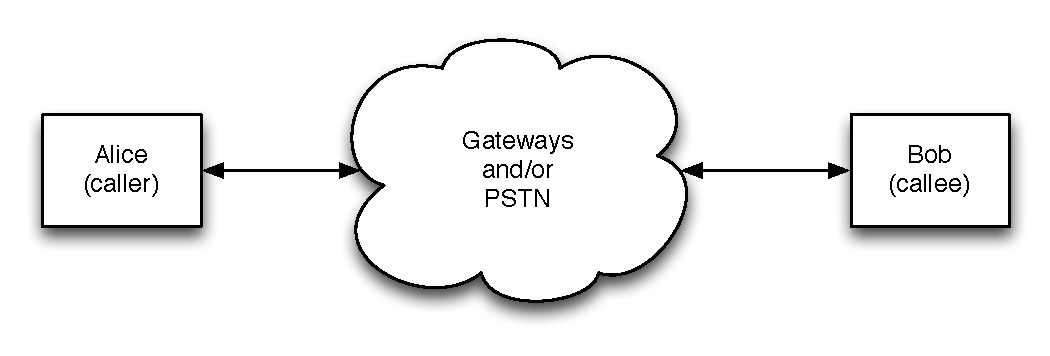
\includegraphics[width=3.7in]{setting1}
\end{center}
\end{slide}

\begin{slide}
\heading{Alternate Setting}

\begin{center}
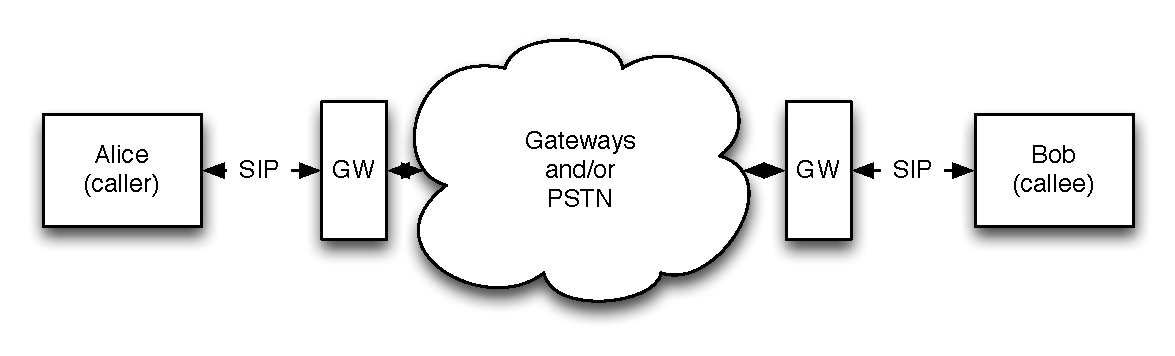
\includegraphics[width=4in]{setting2}
\end{center}
\end{slide}


\begin{slide}
\heading{Assumptions (see Jon's talk)}

\begin{itemize}
\item Endpoints are programmable
  \begin{itemize}
  \item User has a smartphone, softphone, etc.
  \item User has a dumb phone but is serviced by a programmable gateway
  \end{itemize}

\item Very restricted VoIP channel between endpoints
  \begin{itemize}
  \item Effectively just a PSTN call
  \item Caller cannot reliably control caller-id information (CIN field)
  \end{itemize}

\item Each caller ID (e.g., E.164) is associated with cryptographic credentials
  \begin{itemize}
  \item Usable for encryption, authentication, etc.
  \end{itemize}
\end{itemize}
\end{slide}



\begin{slide}
\heading{Credentials}

\begin{itemize}
\item This assumes that each phone number is associated with credentials
\item Requirements
  \begin{itemize}
  \item Bind an E.164 number to key(s)
  \item Suitable for both encryption and authentication
  \item Possible to quickly retrieve the credentials for any number
  \end{itemize}

\item Example: a public key certificate with the E.164 number as subject
\end{itemize}
\end{slide}


\begin{slide}
\heading{System Architecture}

\begin{center}
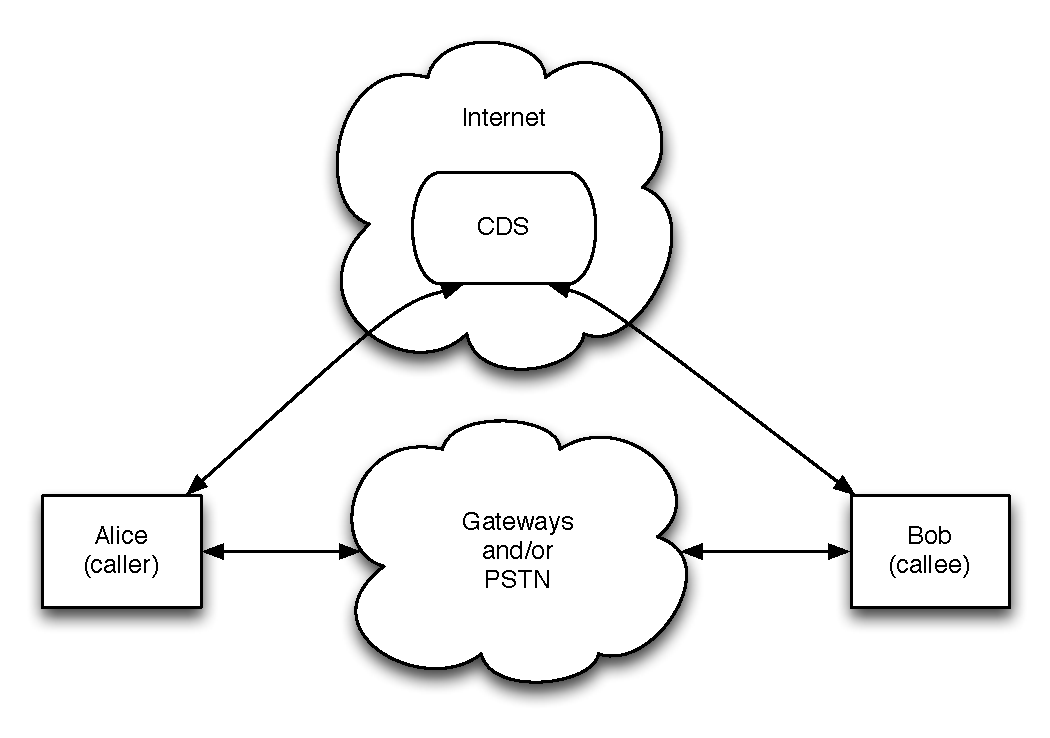
\includegraphics[width=3in]{system}
\end{center}
\end{slide}


\begin{slide}
\heading{Call Flow}

\vspace{-.4in}
\footnotesize{
$$
\xymatrix@C=.8in@R=.2in{
\txt{Alice\\\texttt{1.111.111.1111}} & \txt{Call Detail Service} & \txt{Bob\\\texttt{1.222.222.2222}} \\
\ar@{<->}[r]^{\txt{Authenticate as \texttt{1.111.111.1111}}} & & \\
\ar[r]^{\txt{Store \texttt{E(1.222.222.2222,1.111.111.1111)}}} & & \\
\ar[rr]^{\txt{Call from \texttt{1.111.111.1111}}} & & \\
& & \ar[l]_{\txt{Retrieve CDR from \texttt{1.111.111.1111}}} \\
& \ar[r]^{\txt{\texttt{E(1.222.222.2222,1.111.111.1111)}}} & \\
& & *[l]{\txt{[Call from \texttt{1.111.111.1111}]}}\\
}
$$
}

* Note: $E(X, Y)$ means encrypt ``Y'' for ``X''
\end{slide}



\begin{slide}
\heading{Caller Behavior}

\begin{itemize}
\item Look up callee's credentials (may be cached)
\item Sign and encrypt CDR for callee\symbolfootnote[1]{Special formats needed; must not contain recipient's identity in the clear.}
\item Contact the CDS
  \begin{itemize}
  \item Authenticate as the caller
  \item Store encrypted CDR
  \end{itemize}
\item Initiate call to callee
\end{itemize}
\end{slide}


\begin{slide}
\heading{CDS Behavior}

\begin{itemize}
\item Only store credentials from authorized callers
  \begin{itemize}
  \item This prevents spamming the CDS
  \end{itemize}

\item Provide CDR to any responder
\item What if no CDR exists?
  \begin{itemize}
  \item Generate a random CDR(s)
  \item This helps mask the calling rate
    \begin{itemize}
    \item Though not so well for high-rate callers such as call centers
    \end{itemize}
  \end{itemize}
\end{itemize}
\end{slide}

\begin{slide}
\heading{Callee Behavior}

\begin{itemize}
\item Retrieve encrypted CDR from CDS using claimed caller number
\item Decrypt CDR using private key
\item Verify CDR signature matches caller's alleged identity
\item Check timestamp for relevance (replay prevention)
\end{itemize}
\end{slide}


\begin{slide}
\heading{What are the security guarantees?}

\begin{itemize}
\item There exists a relatively recent call from caller to callee
  \begin{itemize}
  \item Assuming credentials not compromised, etc.
  \end{itemize}

\item No guarantee that it is \emph{this} call
\item This defends against robocalling but not MITM attacks
\end{itemize}

\end{slide}


\begin{slide}
\heading{Substitution Attack}

\vspace{-.4in}
\footnotesize{
$$
\xymatrix@C=.6in@R=.2in{
\txt{Attacker} & \txt{Callback\\Service} & \txt{CDS} & \txt{Bob} \\
\ar[r]^{\txt{Place call to Bob}} & \\
& \ar[r]^{\txt{Store CDR for \texttt{CS}}} & & \\
\ar[rrr]^{\txt{Call from \texttt{CS} (forged ID)}} & & & \\
& \ar[rr]^{\txt{Call from \texttt{CS}}} & & \txt{[Ignored]} \\
& & & \ar[l]_{\txt{Retrieve CDR from \texttt{CS}}} \\
& & \ar[r]^{\txt{CDR from \texttt{CS}}} & \\
& & & *[l]{\txt{[Call from \texttt{CS}]}}\\
}
$$
}       
\end{slide}


\begin{slide}
\heading{Privacy Properties I: Off-path Attackers}

\begin{itemize}
\item Cannot determine anything about who is calling who
\item Cannot determine how many calls a callee is getting
\item Limited information about how many calls a caller is generating
  \begin{itemize}
  \item By polling caller number
  \item Can tell if it is more than the minimum number of fake CDRs the CDS generates
  \end{itemize}
\end{itemize}
\end{slide}


\begin{slide}
\heading{Privacy Properties II: On-path Attackers (to CDS)}

\begin{itemize}
\item Cannot directly tell who is calling who
  \begin{itemize}
  \item Assuming communications to CDS are encrypted
  \end{itemize}

\item If call volumes are low, can do traffic analysis
  \begin{itemize}
  \item Alice and Bob both contacted the CDS within a few seconds
  \end{itemize}

\item Can measure call volumes for caller and callee
  \begin{itemize}
  \item Unless they are hidden behind some kind of proxy (Tor, etc.)
  \end{itemize}
\end{itemize}
\end{slide}


\begin{slide}
\heading{Privacy Properties III: CDS}

\begin{itemize}
\item Anything an on-path attacker can do
\item Can directly measure caller's call volume
\end{itemize}
\end{slide}


\begin{slide}
\heading{Federated CDSs}

\begin{itemize}
\item Don't need to have one giant CDS
\item Each user can select their own CDS
  \begin{itemize}
  \item Indicated in their credentials?
  \item Or delegated from the master CDS?
  \end{itemize}

\item This does not need to be exact
  \begin{itemize}
  \item Callers can fall back (or be bounced) to master CDS during transitions
  \end{itemize}
\end{itemize}

\end{slide}

\begin{slide}
\heading{What about the Credential Service?}

\begin{itemize}
\item All callers and callees need to have credentials
\item Must be possible for any caller to get callee credentials
  \begin{itemize}
  \item Quickly
  \item Somewhat privately
  \item Possible design approaches
    \begin{itemize}
    \item Pre-fetch plus pub-sub
    \item Caching servers/proxies (a la DNS)
    \end{itemize}
  \end{itemize}
\item Caller can provide the callee with his credentials
\end{itemize}
\end{slide}


\begin{slide}
\heading{How important is credential timeliness?}

\begin{itemize}
\item Attacker has caller's credentials
  \begin{itemize}
  \item Can forge calls from attacker
  \end{itemize}

\item Attacker has callee's credentials
  \begin{itemize}
  \item Can poll for calls to callee
  \item But probably only for a small number of callers
  \end{itemize}

\item Compromise versus reassignment?
  \begin{itemize}
  \item Can we not reassign during credential validity window?
  \item This lets us make validity windows longer
  \item Doesn't do anything for compromise
  \end{itemize}

\item What is the minimum detection time?
\end{itemize}
\end{slide}



% \begin{slide}
% \heading{Escalation to VoIP}

% \begin{itemize}
% \item Everything here has assumed that calls are carried through PSTN
%   \begin{itemize}
%   \item What about VoIP?
%   \item Provides more features and better security (See Jon's talk)
%   \end{itemize}

% \item CDRs can contain more than just the caller/callee number
%   \begin{itemize}
%   \item For instance, a SIP URI
%     \begin{itemize}
%     \item Similar concept to VIPR
%     \end{itemize}
%   \end{itemize}

% \item How aggressive should we be about this kind of upgrade?
% \end{itemize}
% \end{slide}



% \begin{slide}
% \heading{Why not store under callee's number? (Barnes)}

% \begin{itemize}
% \item No need for CDS to verify caller
% \item Avoids trial decryption stage
% \item Hard to avoid spamming of CDS
%   \begin{itemize}
%   \item Could be mitigated by authenticated proxies?
%   \end{itemize}

% \item Doesn't let callee control privacy properties
%   \begin{itemize}
%   \item If caller doesn't use a proxy then CDS can do traffic analysis
%   \end{itemize}
% \end{itemize}
% \end{slide}


\begin{slide}
\heading{Why not...?}

\vspace{-.2in}
\begin{itemize}
\item Insert a correlation token in the caller's number
  \begin{itemize}
  \item Could use it to store CDR
  \item Assumed not to be possible
  \end{itemize}

\item Store under a hash of the caller's number
  \begin{itemize}
  \item Better privacy but requires sending more traffic from CDS $\rightarrow$ callee
  \end{itemize}

\item Store under a hash of the caller + callee's number
  \begin{itemize}
  \item May make privacy situation worse
  \item Unless hash is shorter than either number
  \item Very weak if either side is known
  \end{itemize}

\item Is there a practical Private Information Retrieval (PIR) protocol we can use here?
\end{itemize}

\end{slide}

\begin{slide}
\heading{Questions?}
\end{slide}

\end{document}